\documentclass{article} 
\usepackage[marginparwidth=1.7in,top=0.5in,bottom=0.5in,right=2in,left=0.5in]{geometry} 
\usepackage{xcolor} 
\usepackage{mwe}
\usepackage{wrapfig}
\usepackage{tikz} 
\usepackage{multicol}

\usetikzlibrary{automata} 

\pagecolor{yellow!10} 

\title{A Markovian Modeling method For Genomic Data Reduction
and Matching (PROPOSAL)} 
\author{Micah Andrew Thornton} 
\date{\today} 

\begin{document} 
\newgeometry{left = 1 in, right = 1in, top = 3 in, bottom = 2 in}
\begin{titlepage} 
\maketitle{}
\end{titlepage} 

\restoregeometry 

\section{Motivation} 

\marginpar{ The amount of genetic information in the human body (accounting for all cell-cell variations like SNPs) is approximately 150 Zettabytes}


In genomic data analysis, the wealth and abundance of 
available genetic information in human readable format 
is immense (even for just a single lowly organism type 
such as Homo \textit{sapiens}).  The use of Markov Chains, 
which are simple stochastic devices used to represent the 
transition probabilities from state to state in a chaotically
evolving system - one in which updates occur according to some
random mechanism, has been used to help identify certain 
microbial genes \cite{salzberg1998microbial}.  This is probably
the most relevant of the papers describing the application of 
these models to genomic sequences.  In this work the researchers
were able to identify genes using interpolated Markov Models.  
That is an incredibly useful thing to do, and could actually be 
quite simply implemented using the methodology described herein, 
which I believe to be slightly different. 

\section{Methodology}

The primary algorithm that will be used in this project will 
be a simple lexical scanner for $k$-mers in either a sliding 
or a windowed method.  I will write the code in a dialect of 
C so that it is quick to run and scan a sequence, or multiple 
sequences into their equivalent Markovean representation.  
\marginpar{Part of the beauty of the algorithm for estimating 
transition probabilites is that it can be accomplished in real 
time as a sequence is read, meaning that if it turns out to be 
a valuble data reduction technique, then actual full sequences 
will not need to be stored.}
\begin{wrapfigure}{r}{9 cm} 
	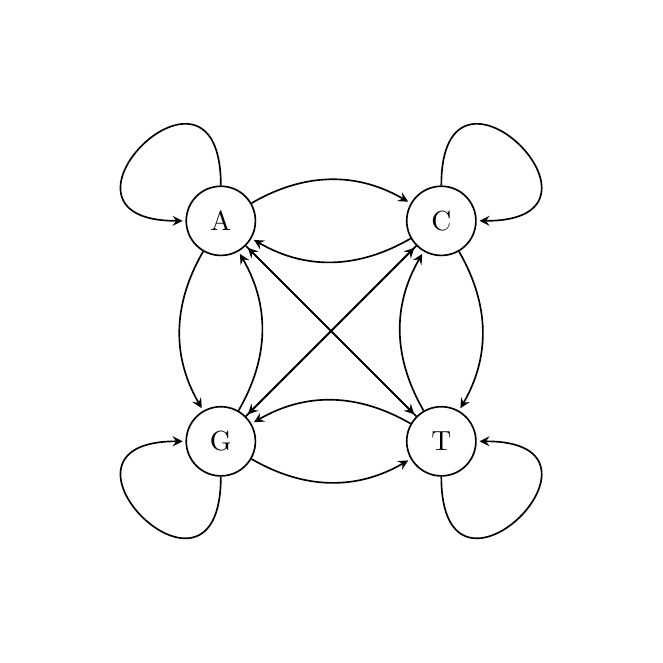
\begin{tikzpicture}[->,>=stealth,shorten >=1pt,auto,node distance=2.8cm,semithick] 
		\node[state] (A) {A}; 
		\node[state] (C)[right of=A] {C}; 
		\node[state] (G)[below of=A] {G}; 
		\node[state] (T)[right of=G] {T}; 
		\path
		(A) edge[in=180,out=90,loop] (A)
		    edge[bend left] (C)
		    edge[bend right] (G) 
		    edge(T)
		(C) edge[in=0,out=90,loop]  (C)
		    edge[bend left] (T) 
		    edge[bend left]  (A) 
		    edge (G)
		(G) edge[in=180,out=270,loop] (G)
		    edge[bend right] (A) 
		    edge[bend right] (T) 
		    edge (C) 
		(T) edge[bend right] (G) 
		    edge[in=0,out=270,loop] (T) 
		    edge[bend left] (C) 
		    edge (A);
	\end{tikzpicture}

	\label{fig:genChain}
	\caption{Generic Markov Chain Representing Single Base Transitions}
\end{wrapfigure}


Consider the diagram of a general chain that is represented 
in Figure \ref{fig:genChain}, whose Probability transition
matrix may be expressed as a four by four matrix of 
sixteen probabilities (floating point - 32 bit or 64 bit values)
that may be estimated for any gene, genomic sequence, etc.  Note
that the chain in figure one is simply an illustration of the
possible configurations.  You may wish to scan through the 
sequence inspecting two base pairs at a time, in which case there 
become 256 probabilities which must be estimated in order to 
complete the chain.  
\marginpar{An $n$-gram is a sequence of $n$ symbols in a row,
such as a sequence of words, a word itself as a sequence of 
characters}
For inspecting three pairs at a time the 
number of probabilities to estimate becomes 4096.  In general 
if we wish to determine the total number of possible transitions
for $n$-grams of length $n$ of symbols from an alphabet of 
cardinality $\Lambda$ than the number of transitions possible $N$ 
is expressed as: 

$$ 
N = \Lambda^{2n}
$$

\section{Utility and Verification} 

There are already methods for assessing sequence similarity, but 
the method laid out in this brief proposal may allow the same, 
finding estimates of the transition probabilities is the key 
in this case, but if transition probabilities can be found, then
confidence intervals can be computed, and then a ratio of the 
number of overlapping confidence intervals may be used as a 
direct measure of the probability of a match.  If we threshold 
probabilities and then compare to known data we can determine 
whether an appropriate match is found or not.  Furthermore, 
methods for taking these matricies and rebuilding the sequence
from which they came could be investigated (such as using a 
combination of a probabilistic/biological model) to recreate
the structure given a few of these matricies. 

Say for instance you had matricies built on single BP transitions, 
double BP transitions, and triple BP transitions alone, then you 
could quickly come up with estimates of the next base pair in 
the sequence given the previous ones, and combining information 
from all chains.  The mathematics here seem pretty sophisticated 
and may take a while to develop, but its possible this could 
result in a quick way to store genetic signals, recreate them with
some error, then go through and do error detection/ correction,
just like the tiny little molecules that parse the DNA strands in
our body do.

\bibliographystyle{plain} 
\bibliography{k} 

\end{document} 
